\documentclass{article}





\usepackage[utf8]{inputenc} % allow utf-8 input
\usepackage[T1]{fontenc}    % use 8-bit T1 fonts
\usepackage{hyperref}       % hyperlinks
\usepackage{url}            % simple URL typesetting
\usepackage{booktabs}       % professional-quality tables
\usepackage{amsfonts}       % blackboard math symbols
\usepackage{nicefrac}       % compact symbols for 1/2, etc.
\usepackage{microtype}      % microtypography
\usepackage{lipsum}		% Can be removed after putting your text content
\usepackage{listings}
\usepackage{url}
\usepackage{graphicx}
\usepackage{longtable}

\lstset{
   basicstyle=\ttfamily\footnotesize
}

\title{Google Gmail Smart Compose}

%\date{September 9, 1985}	% Here you can change the date presented in the paper title
%\date{} 					% Or removing it

\author{
  Giovanni Jiayi Hu\\
  Department of Mathematics\\
  University of Padua, Italy I-35121\\
  \texttt{Email: giovannijiayi.hu@studenti.unipd.it} \\
  %% examples of more authors
  %% \AND
  %% Coauthor \\
  %% Affiliation \\
  %% Address \\
  %% \texttt{email} \\
  %% \And
  %% Coauthor \\
  %% Affiliation \\
  %% Address \\
  %% \texttt{email} \\
  %% \And
  %% Coauthor \\
  %% Affiliation \\
  %% Address \\
  %% \texttt{email} \\
}

% Uncomment to remove the date
%\date{}

% Uncomment to override  the `A preprint' in the header
\renewcommand{\headeright}{}
\renewcommand{\undertitle}{Technical Report}

\begin{document}
\maketitle

\begin{abstract}
This report describes an educational implementation of Gmail Smart Compose which predicts email completion within the browser application. The training involves the Enron email dataset and a sequence-to-sequence model implemented in Keras and then used within the browser with Tensorflow.js .
\end{abstract}


% keywords can be removed
% \keywords{First keyword \and Second keyword \and More}

\section{Gmail Smart Compose}\label{gmail-smart-compose}

Gmail Smart Compose \cite{gmail-smart-compose} is a feature introduced in the popular Google email service back in 2018, which helps to save time on repetitive writing by suggesting relevant contextual phrases. In this report, I explore the approach taken to reproduce a Proof-of-Concept implementation of the same feature using the Enron Email Dataset \cite{kaggle}.

\subsection{Previous work}\label{previous-work}

As the first step into the task, I searched for some information about the technical implementation. The Google Teams published a paper called "Gmail Smart Compose: Real-Time Assisted Writing" \cite{paper} in July 2019 covering much of the challenges and implementation details needed to try to experiment it on my own.

An additional article "Building Gmail style smart compose with a char ngram language model" \cite{building-gmail} from the Machine Learning community helped to gather additional information and implementation details.

Then most of the code contributions came from the official Keras documentation for sequence-to-sequence models: "A ten-minute introduction to sequence-to-sequence learning in Keras" \cite{ten-minutes} and "Sequence to sequence example in Keras (character-level)" \cite{seq2seq-keras}.

\subsection{Environment limits}\label{environment-limits}

The project has been developed mainly using the Colab free plan, thus subject to the limit of 13GB RAM. Also, because of the educational purposes of the project, I aimed for training time within the range of 30-60mins.

\section{Architecture}\label{architecture}

The fundamental task in Smart Compose is to predict a sequence of tokens of variable length, conditioned on the prefix token sequence typed by a user and additional contextual information. During training, the objective is to maximize the log probability of producing the correct target sequence given the input for all data samples in the training corpus.

\subsection{Data}\label{data}

The biggest public email dataset available is the Enron email dataset, which contains approximately 500,000 emails generated by employees of the Enron Corporation. It was obtained by the Federal Energy Regulatory Commission during its investigation of Enron's collapse. Despite its relatively big size (Google trained their models on billions of emails), the usage of this dataset has faced different challenges.

\subsubsection{Previous email}

An important information for the prediction of the completion is the content of the previous email in case the composed one is a response. Unfortunately, the Enron dataset is a flatten set of emails with no information about conversations other than the subject, such ash \texttt{Re:\ hello}. The subject, however, is too fragile to use to safely group emails as related, and it's also often missing as value within the samples. According to the paper, merely joining the subject and the previous email to the model input reduces the log perplexity (the metric used to evaluate the models) is reduced by 0.13, which is a significant improvement.

Another important consequence is that the only relevant information to use as input of the model is the sentence the user is composing.

\subsubsection{Preprocessing}

Preprocessing was a very important step of the project and required careful handling. This is the biggest difference I experienced compared to usual tutorials or exercises, where the dataset is just loaded, and it's already prepared for the task.

The emails are tokenized into words and essential punctuation marks like \texttt{.\ ?\ !\ ,\ '}. Other special marks like new lines are removed and multiple white spaces are compacted as single whitespaces.

Quoted and forwarded messages are removed from the dataset, along with emails longer than 100 words. The latter removal has been done for two purposes: long emails tend to be uncommon to be written again by the user and the increase the required memory and training time by a great amount. Likewise, sentences longer than 20 words are not considered. The model is aimed to learn common sentences which are usually below the threshold of 20 words.

This process resulted in approximately 57 000 sentences.

\subsubsection{Data sequences}

In order to generate the context of a sentence, we train the sequence-to-sequence model to predict the sentence completion from pairs of split sentences of variable length. For instance, the sentence \texttt{here\ is\ our\ forecast} is split in the following pairs within the dataset:

\begin{lstlisting}
[
   ('<start> here is <end>', '<start> our forecast <end>')
   ('<start> here is our <end>', '<start> forecast <end>')
   ('<start> way to <end>', '<start> go !!! <end>')
   ('<start> way to go <end>', '<start> !!! <end>')
   ('<start> let's shoot <end>', '<start> for tuesday at . <end>')
   ('<start> let's shoot for <end>', '<start> tuesday at . <end>')
   ('<start> let's shoot for tuesday <end>', '<start> at . <end>')
   ('<start> let's shoot for tuesday at <end>', '<start> . <end>')
]
\end{lstlisting}

Unique tokens \texttt{\textless{}start\textgreater{}} and \texttt{\textless{}end\textgreater{}} are added to delimit the limits on the input and output sequences. This is both similar to usual Neural Machine Translation (NMT) where the model is given the task to predict from the input sequence \texttt{\textless{}start\textgreater{}\ The\ weather\ is\ nice\ \textless{}end\textgreater{}} the output sequence \texttt{\textless{}start\textgreater{}\ Il\ fault\ beau\ \textless{}end\textgreater{}}

This resulted in approximately 500 000 pairs of sequences.

\subsubsection{Tokenization}

The previous text corpora are transformed into sequences of integers (each integer being the index of a token in a dictionary) by using Keras \texttt{Tokenizer}. I also put a limit to the 10k most frequent words, deleting uncommon words from sentences. This reduces the number of parameters needed to learn in the model and thus the training time.

Sequences are then padded to have the same length, shuffled to avoid pairs from the same sentence to be contiguous, and they are finally ready to be served to the neural model.


\subsection{Natural Language Model}\label{natural-language-model}

Considering the limits of the available dataset, as mentioned in the previous section, the project used the Sequence-to-Sequence Model (seq2seq) similar to NMT, where the source sequence is the start of the sentence and the target sequence the completion. The original paper also uses an attention mechanism to provide better a understanding of the context, but it has been left as potential improvement of the project.

\subsubsection{Training model}\label{training-model}

The following image provides an overview of the final seq2seq model used for training. At its core, it's an Encoder-Decoder model which uses GRU units to encode the input context as in Figure \ref{model}.

\begin{figure}[htbp]
\centering
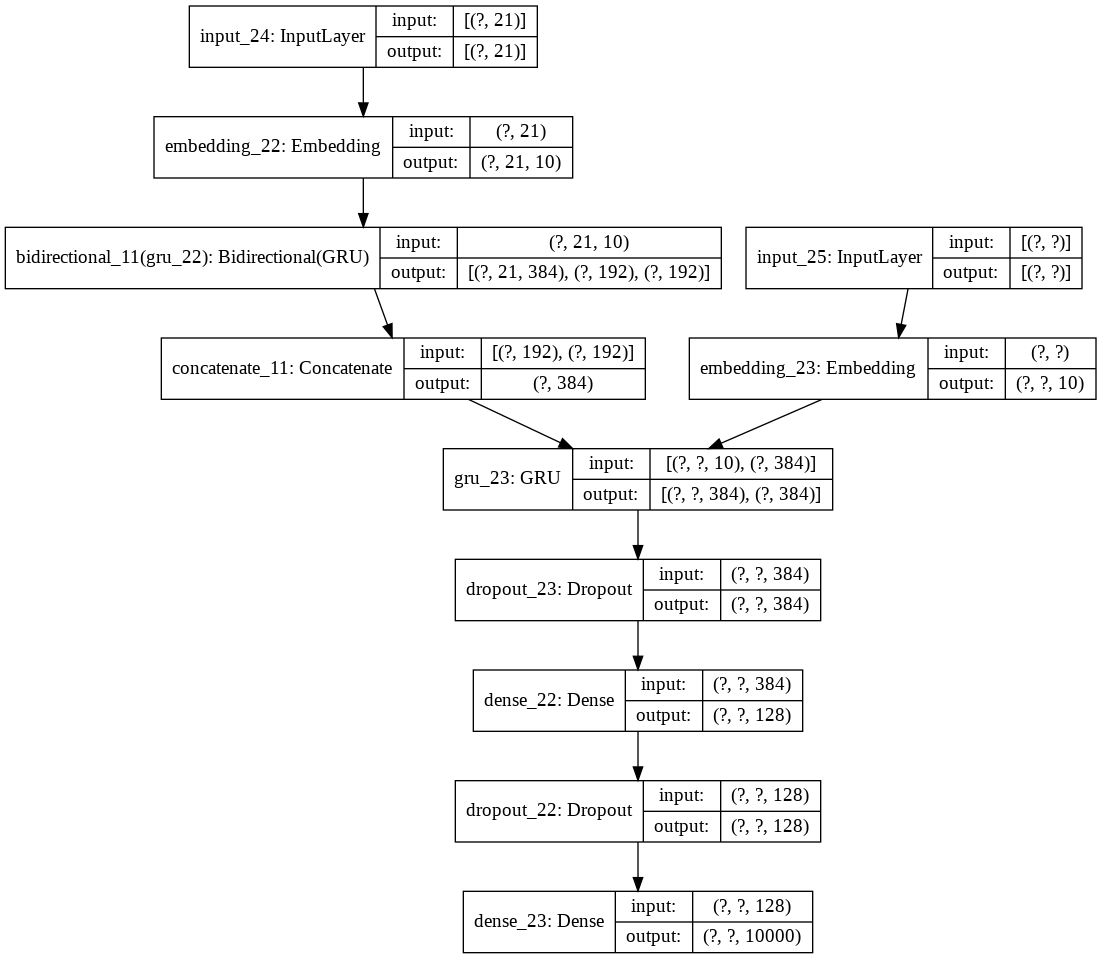
\includegraphics[width=4in]{images/model.png}
\caption{The layers of the seq2seq model}
\label{model}
\end{figure}

\begin{itemize}
\item
  The first layer takes as input the start of the sentences as sequences of integers returned by the \texttt{Tokenizer}and padded to have the same length, 21 integers.
\item
  An embedding layer is used to improve the training. The dimension is set as 10 by following the general advice of using $vocabulary\_size^{0.25}$ as embedding size as suggested in "Introducing TensorFlow Feature Columns" \cite{embedding-size}. The main motivation of the usage of an embedding layer is to introduce the ability to recognize that two sequences are similar without losing the ability to encode both sequences as distinct from the other, while sharing the statistical strength between the two of them and their context. For instance, the two sequences \texttt{Have\ a\ great} and \texttt{Have\ a\ good} should have the same completion \texttt{\textless{}start\textgreater{}\ weekend\ \textless{}end\textgreater{}}.
\item
  The Encoder is comprised of a Bidirectional Gated Recurrent Units (GRU) layer. GRU units have been used as a gating mechanism to better encode the input sequences compared to common RNN. The latter suffers the vanishing gradient issue, especially with the case of the sequences in this dataset which reach a length of 20 words. Compared instead to Long short-term memory (LSTM) units, GRU units have been proved in practice to perform better with the task under consideration. Furthermore, GRU units have only one state, the Hidden State, whereas an Encoder with LSTM units requires working with both the Hidden States and the Cell states. Finally, since the usage of the Bidirectional model, both the forward and backward Hidden States are concatenated to form a single Encoded Hidden State.
\item
  During the training, the model uses \textbf{teacher forcing} as shown in Figure \ref{autoencoder-training}. Specifically, it is trained to turn the target sequences into the same sequences but offset by one time-step in the future. After the model is trained, the \texttt{\textless{}start\textgreater{}} token can be used to start the process and the generated word in the output sequence is used as input on the subsequent time step. However, during the training, we obtain values which are likely to be different from the ground truth and they set the model off track because every subsequently generated word will be based on a wrong history. For this reason, during the training, the model receives the ground truth output $y^t$ as input at time \texttt{t\ +\ 1}. This explains the usage of an additional Input Layer and Embedding, containing the ground truth sequence.

  \begin{figure}[htbp]
   \centering
   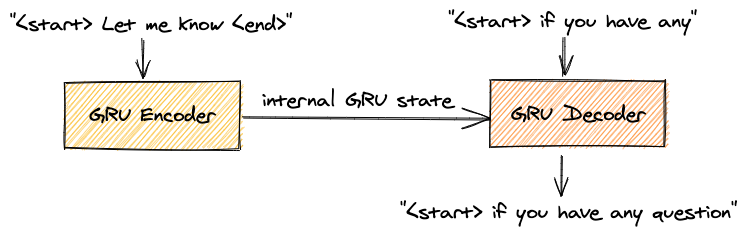
\includegraphics[width=5in]{images/autoencoder-training}
   \caption{Teacher forcing during training}
   \label{autoencoder-training}
   \end{figure}
\item
  The Decoder is comprised of a GRU layer which takes as input the Encoded Hidden State and the ground truth output from the previous time-step. Then a Dropout layer is added to its output to avoid overfitting, and an additional Dense layer is used to improve inference capabilities. Finally, the last Dense layer produces the logits for each word in the dictionary, assigning to each of them a probability of being the correct word to predict. Since the categories are provided as integers, the function used as loss is \texttt{sparse\_categorical\_crossentropy} whereas \texttt{perplexity} is the metric.

  $$Perplexity(x) = -\sum_x{p(x)\ log\ p(x)}$$

  $x$ is the ground truth label and $p(x)$ is the model. The lower is the perplexity, and the higher is the probability of assigning the true target tokens. Perplexity is a typical metric used to evaluate language model and it's the same used in the Google paper.
\end{itemize}

In Table \ref{tab:hyperparameters} the results of different architectures or hyper-parameters.

\begin{table}[!htbp]
   \centering
   \begin{tabular}{lccc}
     \toprule
     Architecture & \# Parameters & Training time & Perplexity \\
     \midrule
     Bidirectional GRU 128 outputs with a Decoder Dense Layer of 128 units & 1,836,240 & 34min & 1.8793 \\
     Bidirectional LSTM 128 outputs with a Decoder Dense Layer of 128 units & 1,938,640 & 43min & 1.9327 \\
     Forward-only GRU 128 outputs with a Decoder Dense Layer of 128 units  & 1,614,032 & 24min & 2.0357 \\
     Bidirectional GRU 128 outputs with a Decoder Dense Layer of 256 units & 3,149,136 & 61min & 1.6835 \\
     \bottomrule
   \end{tabular}
   \caption{Results of different model hyperparameters or memory units}
   \label{tab:hyperparameters}
\end{table}

Despite the best model is 128 GRU units with 256 units in the hidden Dense layer, the model has much more parameters and therefore incurs also in slower inference time later. Since inference latency is an important metric for the task under consideration, I preferred to keep 128 units in the hidden layer which is the secondo best-scoring model.

\subsubsection{Inference Model}\label{inference-model}

During the inference, the model uses separately the Encoder to encode the input sequence whereas the Decoder will not be fed with the true output and it's approximated with the model's output at the previous time-step as shown in Figure \ref{autoencoder-inference}.

\begin{figure}[htbp]
\centering
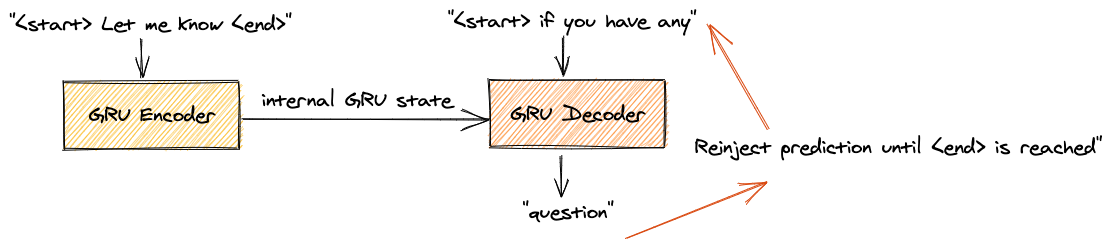
\includegraphics[width=7in]{images/autoencoder-inference}
\caption{Prediction re-injected during inference}
\label{autoencoder-inference}
\end{figure}

The Encoder in Figure \ref{encoder} uses the same layers of the training Encoder-Decoder.

\begin{figure}[htbp]
\centering
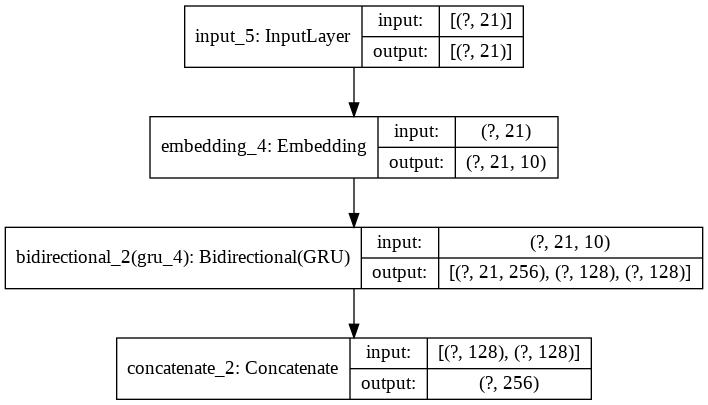
\includegraphics[width=4in]{images/encoder.png}
\caption{The Inference Encoder}
\label{encoder}
\end{figure}

Likewise, the Inference Decoder in Figure \ref{inf-model} uses the same layers as before, with the only difference that it uses the word predicted at the previous step as input along with the Encoded Hidden State.

\begin{figure}[htbp]
\centering
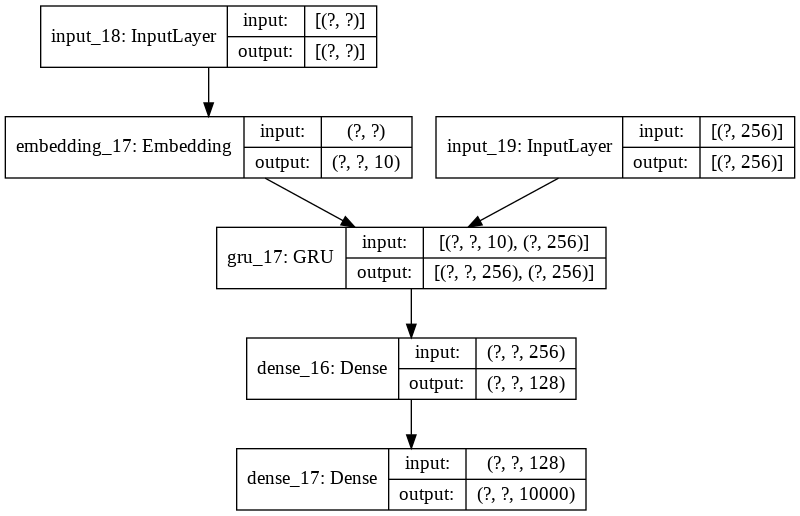
\includegraphics[width=4in]{images/inf-model.png}
\caption{Layers in the Inference Decoder model}
\label{inf-model}
\end{figure}

The inference Decoder predicts the sentence completion by doing the following steps:

\begin{enumerate}
\item
  It tokenizes and embeds the input sequence using the same preprocessing of the training inputs
\item
  The Encoder returns the Encoded Hidden State
\item
  The target sequence starts with only the \texttt{\textless{}start\textgreater{}} token and is conditioned to generate an output work token based on the context provided by the Encoded Hidden State. The
\item
  Step 3 is repeated until the token \texttt{\textless{}end\textgreater{}} is generated. The final sequence is converted back from integer tokens to words using the reverse dictionary of the \texttt{Tokenizer}.
\end{enumerate}

\section{Evaluation}\label{evaluation}

Below there are some results provided by the inference.

\begin{table}[!htbp]
   \centering
   \begin{tabular}{ll}
     \toprule
     Input & Output \\
     \midrule
     here is & the latest version of the captioned schedule . <end> \\
     have a & great weekend <end> \\
     please review & the attached outage report <end> \\
     please call me & if you have any questions <end> \\
     thanks for & the info <end> \\
     let me & know if you have any questions <end> \\
     Let me know & if you have any questions <end> \\
     Let me know if you & have any questions <end> \\
     this sounds & like the final four tickets is attached <end> \\
     is this call going to & have a meeting ? <end> \\
     can you get & a copy of the equitrans agreement next week ? thanks <end> \\
     is it okay & ? <end> \\
     it should & be the final ge <end> \\
     call if there's & have any questions <end> \\
     gave her a & call <end> \\
     i will let & you know <end> \\
     i will be & out of the office until monday , january , . <end> \\
     may i get a copy of all the & invoices <end> \\
     how is our trade & ? <end> \\
     this looks like a & bit <end> \\
     i am fine with the changes & . <end> \\
     please be sure this & is a copy of the attached <end> \\
     \bottomrule
   \end{tabular}
   \caption{Input-Output predictions of the inference model}
\end{table}

The predicted outputs are actually quite good. The inference model is especially good with short common sentences like \textit{"Let me know if you have any questions"} or \textit{"I will let you know"}. Some predictions also show that the predictions are personalized based on the Enron dataset, for instance in the case of \textit{"here is the latest version of the captioned schedule"}.

Unfortunately, some other cases such as \textit{"it should be the final ge"} or \textit{"i will be out of the office until monday , january , ."} seem to be a bit off because of the preprocessing. If we had a bigger dataset and more training time this completions should have been discarded as very unlikely to be correct.

\section{Inference in the browser}\label{inference-in-the-browser}

Because the model must be used to predict email autocompletion, the next step is to save the model and make the inference on the fly while the user types. This can be done on the server or on directly in the browser. Because of the low-latency requirements and the cost of renting an ever-running server, the decision has been to try using the model within the browser.

For this goal, both the \texttt{Tokenizer} dictionary and the Keras model must be saved and loaded later in the browser. The word-to-integer dictionary is just saved as JSON, whereas I found that \texttt{H5} is the best working format for the Keras model. Attempts to use the Tensorflow \texttt{SavedModel} \cite{saved-model} resulted in errors while converting the model to the web using \texttt{tensorflowjs-converter} \cite{model-conversion}.

The model is then loaded in the browser along with the pre-trained weights using \texttt{Tensorflow.js} \cite{tensorflowjs}, a JavaScript implementation of the framework. In particular, because JavaScript executes in a single main thread shared with UI rendering, in order to avoid freezing the page while loading the model or during the inference calculations, all the Keras processing is done in a separate thread via \texttt{Web Worker} \cite{web-worker} as shown in Figure \ref{keras-web-worker}.

The main thread communicates with the Web Worker via messages, and the latter executes the tokenization of the input sequence and the subsequent model inference. Then the result is returned to the browser main thread via message again.

\begin{figure}[htbp]
\centering
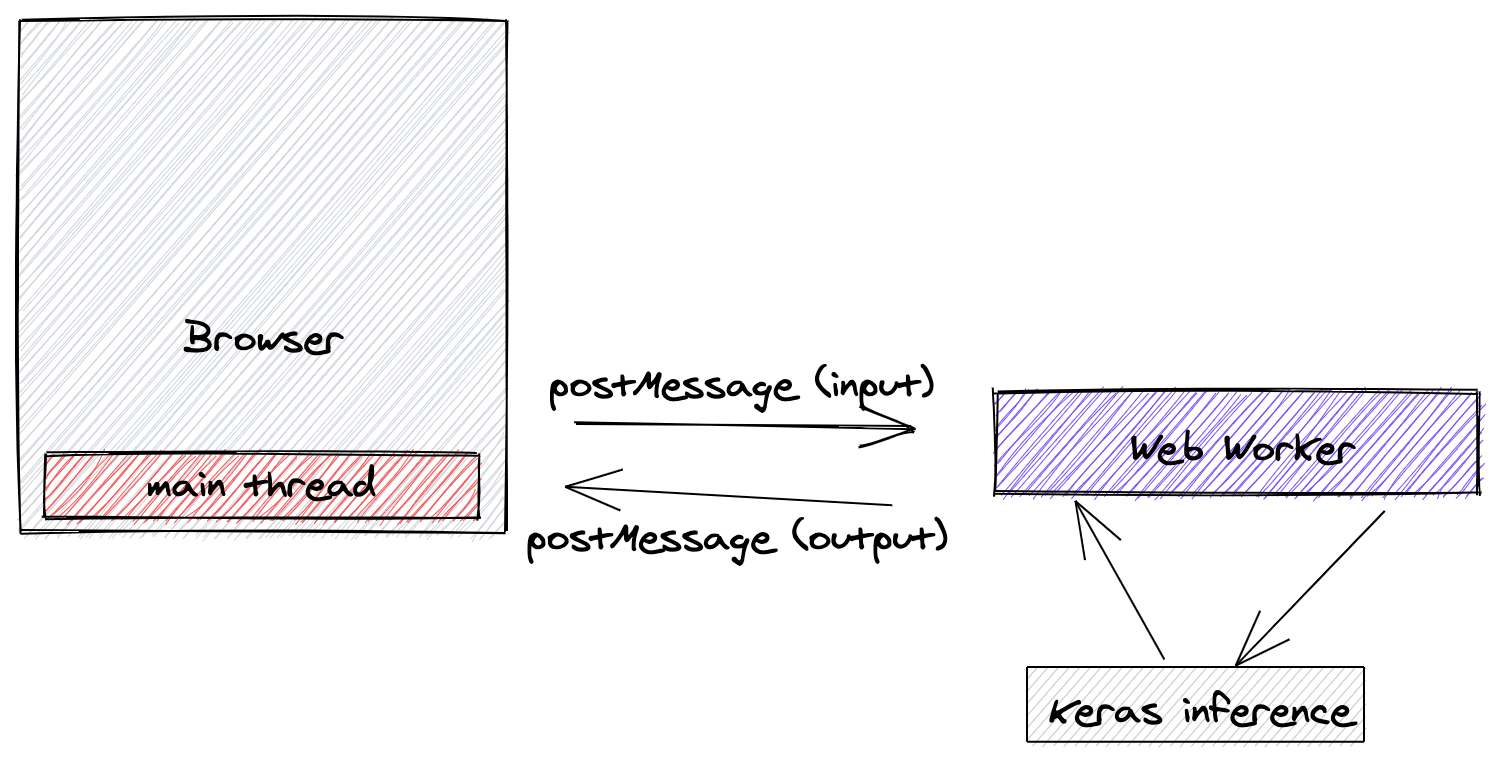
\includegraphics[width=4in]{images/keras-web-worker.png}
\caption{A representation of Model inference in the browser}
\label{keras-web-worker}
\end{figure}

The final source code are available on the repository at \href{https://github.com/jiayihu/gmail-smart-compose}{github.com/jiayihu/gmail-smart-compose}. For easier evaluation, there is also a \href{https://colab.research.google.com/drive/1wjr-Ntnd4zYMneyGUz1beEmyw0fwgnEG?usp=sharing}{notebook on Colab}.

\section{Conclusions}\label{conclusions}

The project has been the first real-world usage of NLP notions and Deep Learning techniques. The most important lessons have been:

\begin{enumerate}
\item
  Before even thinking about the learning model, there is a lot of work that needs to be done during the preprocessing phase. The available dataset to be used as input for the model assumes an important role on the subsequent training and goodness of the results. I would dare to say that data quality is as important as the training model. Unfortunately the Enron dataset is the only meaningful dataset but is lacking important information like linking responses.
\item
  Training real-world models requires a lot of RAM and computing power. The project has been trained using Colab free plan which limits the available RAM to 13GB and there are also limitations on the amount of GPU usage. Although this prohibited the training of more complex models or for a long time, at first it forced me to think better about the data structures I was using and the amount of input used to generate the dataset. I started to be more careful about what to include in the dataset, which resulted in both less RAM usage and more accurate inference predictions. At the same time, there are obviously strongs disadvantages in limited RAM and training time. According to the paper, Google ran their models on billions of emails and for at least 3 days using high-end TPUs. But for educational purposes, 13GB should be enough to learn something meaningful.
\end{enumerate}

\bibliographystyle{unsrt}
%\bibliography{references}  %%% Remove comment to use the external .bib file (using bibtex).
%%% and comment out the "thebibliography" section.


%%% Comment out this section when you \bibliography{references} is enabled.
\begin{thebibliography}{1}

\bibitem{gmail-smart-compose}
\newblock "SUBJECT: Write emails faster with Smart Compose in Gmail". \url{https://www.blog.google/products/gmail/subject-write-emails-faster-smart-compose-gmail/}

\bibitem{kaggle}
\newblock Kaggle - "Enron Email Dataset". \url{https://www.kaggle.com/wcukierski/enron-email-dataset}

\bibitem{paper}
\newblock Mia Xu Chen et al. "Gmail smart compose: Real-time assisted writing". 2019. \url{https://dl.acm.org/doi/abs/10.1145/3292500.3330723}

\bibitem{building-gmail}
\newblock "Building Gmail style smart compose with a char ngram language model". \url{https://towardsdatascience.com/gmail-style-smart-compose-using-char-n-gram-language-models-a73c09550447}

\bibitem{ten-minutes}
\newblock "A ten-minute introduction to sequence-to-sequence learning in Keras". \url{https://blog.keras.io/a-ten-minute-introduction-to-sequence-to-sequence-learning-in-keras.html}

\bibitem{seq2seq-keras}
\newblock "Sequence to sequence example in Keras (character-level)". \url{https://keras.io/examples/lstm_seq2seq/}.

\bibitem{embedding-size}
\newblock "Introducing TensorFlow Feature Columns". \url{https://developers.googleblog.com/2017/11/introducing-tensorflow-feature-columns.html}

\bibitem{saved-model}
\newblock TensorFlow.js. "Using the SavedModel format". \url{https://www.tensorflow.org/guide/saved_model}

\bibitem{model-conversion}
\newblock TensorFlow.js. "Model conversion". \url{https://www.tensorflow.org/js/guide/conversion}

\bibitem{tensorflowjs}
\newblock TensorFlow.js. \url{https://www.tensorflow.org/js}

\bibitem{web-worker}
\newblock Mozilla Developer Network. "Using Web Workers". \url{https://developer.mozilla.org/en-US/docs/Web/API/Web_Workers_API/Using_web_workers}

\end{thebibliography}


\end{document}
